\begin{figure}[t]
    \centering
    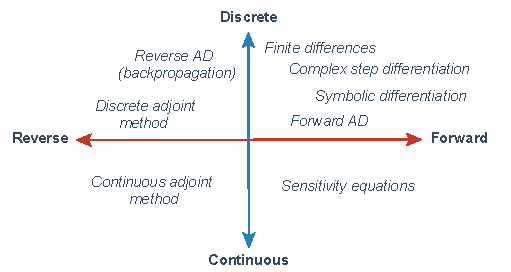
\includegraphics[width=0.80\textwidth]{figures/scheme-methods.pdf}
    \caption{Schematic representation of the different methods available for differentiation involving differential equation solutions. These can be classified depending if they find the gradient by solving a new system of differential equations (\textit{continuous}) or if instead they manipulate unit algebraic operations (\textit{discrete}). Additionally, these methods can be categorized based on their alignment with the direction of the numerical solver. If they operate in the same direction as the solver, they are referred to as \textit{forward} methods. Conversely, if they function in the opposite direction, they are known as \textit{reverse} methods.}
    \label{fig:scheme-all-methods}
\end{figure}

There is a large family of methods for computing gradients or sensitivities of systems of differential equations. 
Depending on the number of parameters and the characteristics of the differential equation we are trying to solve (e.g., level of stiffness), they have different mathematical, numerical, and computational advantages.
These methods can be roughly classified as  follows \cite{ma2021comparison}. 
\begin{itemize}
    \item \textit{Continuous} vs \textit{discrete}  methods
    \item \textit{Forward} vs \textit{reverse} methods
\end{itemize}
Figure \ref{fig:scheme-all-methods} displays a classification of some methods under this two-fold classification. 

The \textit{continuous} vs \textit{discrete} distinction is one of mathematical and numerical nature. 
When solving for the gradient of a differential equation, one needs to derive both a mathematical expression for the gradient (the differentiation step) and solve the equations using a numerical solver (the discretization step) \cite{bradley2013pde, Onken_Ruthotto_2020, FATODE2014, Sirkes_Tziperman_1997}. 
Depending on the order of these two operations, we refer to discrete methods (discretize-then-differentiate) or continuous methods (differentiate-then-discretize). 
In the case of \textit{discrete} methods, gradients are computed based on simple function evaluations of the solutions of the numerical solver (finite differences, complex step differentiation) or by manipulation of atomic operations inside a numerical solver (AD, symbolic differentiation, discrete adjoint method). 
It is worth noting that although both approaches are subsumed under discrete methods, their numerical properties are quite different.
In the case of \textit{continuous} methods, a new set of differential equations is derived for the sensitivity (sensitivity equations) or the adjoint (continuous adjoint method) of the system, both quantities that allow the calculation of the desired gradient.   
% We can either discretize the original system of ODEs in order to numerically solve it and then find an strategy to differentiate it; or instead define new equations for the differentiation step and later numerically solver them.
When comparing discrete to continuous methods, we are focusing, beyond computational efficiency, on the mathematical consistency of the method, that is, \textit{is the method estimating the right gradient?}. 
When using discrete methods, we may have an algorithmically correct method, meaning that it is computing the gradient of the solver discretization, but it is not approximating the gradient of the true solution of the differential equation. 
For example, methods such as automatic differentiation may compute the exact derivative of the numerical approximation of a loss function and yet not give a good approximation of the exact derivative of the loss \cite{Walther_2007}.
However, one has to keep in mind that AD computes the exact derivative of an approximation of the objective and may not yield an approximation to the exact derivatives of the objective (Section \ref{section:forwardAD-sensitivity}).

The \textit{forward} vs \textit{reverse} distinction considers when the gradient is computed, i.e., whether this happens during the forward pass of the numerical solver or in a later recalculation \cite{Griewank:2008kh}. 
In all \textit{forward} methods the solution of the differential equation is solved sequentially and simultaneously with the derivative (either the full gradient or more commonly a directional derivative) during the forward pass of the numerical solver. 
% \todo[inline]{That doesn't sound right, see Griewank, section 3: the forward model computes directional derivatives, not gradients (tangent mode), the reverse mode computes gradients (adjoint mode). I.e., forward mode maps between tangent spaces, reverse mode maps between cotangent spaces. The text can be corrected if you replace "gradient" more generically by "derivative" (but it then misses the point).}
On the contrary, \textit{reverse} methods compute the gradient tracking backwards the forward model by resolving a new problem that moves in the opposite direction as the original numerical solver. 
For systems of ordinary differential equations (ODEs) and initial value problems (IVPs), most numerical methods solve the differential equation progressively moving forward in time, meaning that reverse methods then solve for the gradient moving backwards in time. 

As we will discuss in the following sections, forward methods are very efficient for problems with a small number of parameters we want to differentiate with respect to, while reverse methods are more efficient for a large number of parameters but they come with a larger memory cost or compute overhead which needs to be overcome using different performance tricks. 
With the exception of finite differences and complex step differentiation, the rest of the forward methods (i.e. forward AD, sensitivity equations, symbolic differentiation) compute the full sensitivity of the differential equation, that is, how the full solution of the ODEs changes when we change the parameters of the model. 
This can be computationally expensive or intractable for large systems. 
Conversely, reverse methods are based on the computation of intermediate variables, known as the adjoint or dual variables, that cleverly avoid the unnecessary calculation of the full sensitivity at expenses of larger memory cost \cite{Givoli_2021}. 
% For this reason, reverse methods can be also labeled as adjoint methods \cite{ma2021comparison}. 

% Double-check this paragraph to see if we still want to include it. 
One extra distinction between methods is with regards to how computationally entangled the numerical solver and the differentiation machinery are. 
% With the exception of the discrete adjoint methods, this coincides with discrete-continuous classification. 
However, the construction of the discrete adjoint is based on the numerical solver, something that does not happen with the other discrete methods. 
While this might not have big conceptual implications, it is an important consideration when using software that integrates numerical solvers and differentiation, a distinction that will help in the discussion in Section \ref{sec:computational-implementation}.

The rest of this section is organized as follows. 
We first introduce some basic mathematical notions that are going to facilitate the discussion of the sensitivity methods (Section \ref{section:preliminaries}).
We then mathematically introduce each of the methods listed in Figure \ref{fig:scheme-all-methods}.
We finalize the discussion in Section \ref{section:compatison-math} with a comparison of some mathematical foundations of these methods. 
% More specificlacy, our goal here is try to enlight the closed resamblance of the methods 